% Options for packages loaded elsewhere
\PassOptionsToPackage{unicode}{hyperref}
\PassOptionsToPackage{hyphens}{url}
\PassOptionsToPackage{dvipsnames,svgnames,x11names}{xcolor}
%
\documentclass[
  letterpaper,
  DIV=11]{scrartcl}

\usepackage{amsmath,amssymb}
\usepackage{iftex}
\ifPDFTeX
  \usepackage[T1]{fontenc}
  \usepackage[utf8]{inputenc}
  \usepackage{textcomp} % provide euro and other symbols
\else % if luatex or xetex
  \usepackage{unicode-math}
  \defaultfontfeatures{Scale=MatchLowercase}
  \defaultfontfeatures[\rmfamily]{Ligatures=TeX,Scale=1}
\fi
\usepackage{lmodern}
\ifPDFTeX\else  
    % xetex/luatex font selection
\fi
% Use upquote if available, for straight quotes in verbatim environments
\IfFileExists{upquote.sty}{\usepackage{upquote}}{}
\IfFileExists{microtype.sty}{% use microtype if available
  \usepackage[]{microtype}
  \UseMicrotypeSet[protrusion]{basicmath} % disable protrusion for tt fonts
}{}
\makeatletter
\@ifundefined{KOMAClassName}{% if non-KOMA class
  \IfFileExists{parskip.sty}{%
    \usepackage{parskip}
  }{% else
    \setlength{\parindent}{0pt}
    \setlength{\parskip}{6pt plus 2pt minus 1pt}}
}{% if KOMA class
  \KOMAoptions{parskip=half}}
\makeatother
\usepackage{xcolor}
\setlength{\emergencystretch}{3em} % prevent overfull lines
\setcounter{secnumdepth}{5}
% Make \paragraph and \subparagraph free-standing
\ifx\paragraph\undefined\else
  \let\oldparagraph\paragraph
  \renewcommand{\paragraph}[1]{\oldparagraph{#1}\mbox{}}
\fi
\ifx\subparagraph\undefined\else
  \let\oldsubparagraph\subparagraph
  \renewcommand{\subparagraph}[1]{\oldsubparagraph{#1}\mbox{}}
\fi

\usepackage{color}
\usepackage{fancyvrb}
\newcommand{\VerbBar}{|}
\newcommand{\VERB}{\Verb[commandchars=\\\{\}]}
\DefineVerbatimEnvironment{Highlighting}{Verbatim}{commandchars=\\\{\}}
% Add ',fontsize=\small' for more characters per line
\usepackage{framed}
\definecolor{shadecolor}{RGB}{241,243,245}
\newenvironment{Shaded}{\begin{snugshade}}{\end{snugshade}}
\newcommand{\AlertTok}[1]{\textcolor[rgb]{0.68,0.00,0.00}{#1}}
\newcommand{\AnnotationTok}[1]{\textcolor[rgb]{0.37,0.37,0.37}{#1}}
\newcommand{\AttributeTok}[1]{\textcolor[rgb]{0.40,0.45,0.13}{#1}}
\newcommand{\BaseNTok}[1]{\textcolor[rgb]{0.68,0.00,0.00}{#1}}
\newcommand{\BuiltInTok}[1]{\textcolor[rgb]{0.00,0.23,0.31}{#1}}
\newcommand{\CharTok}[1]{\textcolor[rgb]{0.13,0.47,0.30}{#1}}
\newcommand{\CommentTok}[1]{\textcolor[rgb]{0.37,0.37,0.37}{#1}}
\newcommand{\CommentVarTok}[1]{\textcolor[rgb]{0.37,0.37,0.37}{\textit{#1}}}
\newcommand{\ConstantTok}[1]{\textcolor[rgb]{0.56,0.35,0.01}{#1}}
\newcommand{\ControlFlowTok}[1]{\textcolor[rgb]{0.00,0.23,0.31}{#1}}
\newcommand{\DataTypeTok}[1]{\textcolor[rgb]{0.68,0.00,0.00}{#1}}
\newcommand{\DecValTok}[1]{\textcolor[rgb]{0.68,0.00,0.00}{#1}}
\newcommand{\DocumentationTok}[1]{\textcolor[rgb]{0.37,0.37,0.37}{\textit{#1}}}
\newcommand{\ErrorTok}[1]{\textcolor[rgb]{0.68,0.00,0.00}{#1}}
\newcommand{\ExtensionTok}[1]{\textcolor[rgb]{0.00,0.23,0.31}{#1}}
\newcommand{\FloatTok}[1]{\textcolor[rgb]{0.68,0.00,0.00}{#1}}
\newcommand{\FunctionTok}[1]{\textcolor[rgb]{0.28,0.35,0.67}{#1}}
\newcommand{\ImportTok}[1]{\textcolor[rgb]{0.00,0.46,0.62}{#1}}
\newcommand{\InformationTok}[1]{\textcolor[rgb]{0.37,0.37,0.37}{#1}}
\newcommand{\KeywordTok}[1]{\textcolor[rgb]{0.00,0.23,0.31}{#1}}
\newcommand{\NormalTok}[1]{\textcolor[rgb]{0.00,0.23,0.31}{#1}}
\newcommand{\OperatorTok}[1]{\textcolor[rgb]{0.37,0.37,0.37}{#1}}
\newcommand{\OtherTok}[1]{\textcolor[rgb]{0.00,0.23,0.31}{#1}}
\newcommand{\PreprocessorTok}[1]{\textcolor[rgb]{0.68,0.00,0.00}{#1}}
\newcommand{\RegionMarkerTok}[1]{\textcolor[rgb]{0.00,0.23,0.31}{#1}}
\newcommand{\SpecialCharTok}[1]{\textcolor[rgb]{0.37,0.37,0.37}{#1}}
\newcommand{\SpecialStringTok}[1]{\textcolor[rgb]{0.13,0.47,0.30}{#1}}
\newcommand{\StringTok}[1]{\textcolor[rgb]{0.13,0.47,0.30}{#1}}
\newcommand{\VariableTok}[1]{\textcolor[rgb]{0.07,0.07,0.07}{#1}}
\newcommand{\VerbatimStringTok}[1]{\textcolor[rgb]{0.13,0.47,0.30}{#1}}
\newcommand{\WarningTok}[1]{\textcolor[rgb]{0.37,0.37,0.37}{\textit{#1}}}

\providecommand{\tightlist}{%
  \setlength{\itemsep}{0pt}\setlength{\parskip}{0pt}}\usepackage{longtable,booktabs,array}
\usepackage{calc} % for calculating minipage widths
% Correct order of tables after \paragraph or \subparagraph
\usepackage{etoolbox}
\makeatletter
\patchcmd\longtable{\par}{\if@noskipsec\mbox{}\fi\par}{}{}
\makeatother
% Allow footnotes in longtable head/foot
\IfFileExists{footnotehyper.sty}{\usepackage{footnotehyper}}{\usepackage{footnote}}
\makesavenoteenv{longtable}
\usepackage{graphicx}
\makeatletter
\def\maxwidth{\ifdim\Gin@nat@width>\linewidth\linewidth\else\Gin@nat@width\fi}
\def\maxheight{\ifdim\Gin@nat@height>\textheight\textheight\else\Gin@nat@height\fi}
\makeatother
% Scale images if necessary, so that they will not overflow the page
% margins by default, and it is still possible to overwrite the defaults
% using explicit options in \includegraphics[width, height, ...]{}
\setkeys{Gin}{width=\maxwidth,height=\maxheight,keepaspectratio}
% Set default figure placement to htbp
\makeatletter
\def\fps@figure{htbp}
\makeatother
\newlength{\cslhangindent}
\setlength{\cslhangindent}{1.5em}
\newlength{\csllabelwidth}
\setlength{\csllabelwidth}{3em}
\newlength{\cslentryspacingunit} % times entry-spacing
\setlength{\cslentryspacingunit}{\parskip}
\newenvironment{CSLReferences}[2] % #1 hanging-ident, #2 entry spacing
 {% don't indent paragraphs
  \setlength{\parindent}{0pt}
  % turn on hanging indent if param 1 is 1
  \ifodd #1
  \let\oldpar\par
  \def\par{\hangindent=\cslhangindent\oldpar}
  \fi
  % set entry spacing
  \setlength{\parskip}{#2\cslentryspacingunit}
 }%
 {}
\usepackage{calc}
\newcommand{\CSLBlock}[1]{#1\hfill\break}
\newcommand{\CSLLeftMargin}[1]{\parbox[t]{\csllabelwidth}{#1}}
\newcommand{\CSLRightInline}[1]{\parbox[t]{\linewidth - \csllabelwidth}{#1}\break}
\newcommand{\CSLIndent}[1]{\hspace{\cslhangindent}#1}

\usepackage{booktabs}
\usepackage{longtable}
\usepackage{array}
\usepackage{multirow}
\usepackage{wrapfig}
\usepackage{float}
\usepackage{colortbl}
\usepackage{pdflscape}
\usepackage{tabu}
\usepackage{threeparttable}
\usepackage{threeparttablex}
\usepackage[normalem]{ulem}
\usepackage{makecell}
\usepackage{xcolor}
\KOMAoption{captions}{tableheading}
\makeatletter
\@ifpackageloaded{tcolorbox}{}{\usepackage[skins,breakable]{tcolorbox}}
\@ifpackageloaded{fontawesome5}{}{\usepackage{fontawesome5}}
\definecolor{quarto-callout-color}{HTML}{909090}
\definecolor{quarto-callout-note-color}{HTML}{0758E5}
\definecolor{quarto-callout-important-color}{HTML}{CC1914}
\definecolor{quarto-callout-warning-color}{HTML}{EB9113}
\definecolor{quarto-callout-tip-color}{HTML}{00A047}
\definecolor{quarto-callout-caution-color}{HTML}{FC5300}
\definecolor{quarto-callout-color-frame}{HTML}{acacac}
\definecolor{quarto-callout-note-color-frame}{HTML}{4582ec}
\definecolor{quarto-callout-important-color-frame}{HTML}{d9534f}
\definecolor{quarto-callout-warning-color-frame}{HTML}{f0ad4e}
\definecolor{quarto-callout-tip-color-frame}{HTML}{02b875}
\definecolor{quarto-callout-caution-color-frame}{HTML}{fd7e14}
\makeatother
\makeatletter
\makeatother
\makeatletter
\makeatother
\makeatletter
\@ifpackageloaded{caption}{}{\usepackage{caption}}
\AtBeginDocument{%
\ifdefined\contentsname
  \renewcommand*\contentsname{Inhaltsverzeichnis}
\else
  \newcommand\contentsname{Inhaltsverzeichnis}
\fi
\ifdefined\listfigurename
  \renewcommand*\listfigurename{Abbildungsverzeichnis}
\else
  \newcommand\listfigurename{Abbildungsverzeichnis}
\fi
\ifdefined\listtablename
  \renewcommand*\listtablename{Tabellenverzeichnis}
\else
  \newcommand\listtablename{Tabellenverzeichnis}
\fi
\ifdefined\figurename
  \renewcommand*\figurename{Abbildung}
\else
  \newcommand\figurename{Abbildung}
\fi
\ifdefined\tablename
  \renewcommand*\tablename{Tabelle}
\else
  \newcommand\tablename{Tabelle}
\fi
}
\@ifpackageloaded{float}{}{\usepackage{float}}
\floatstyle{ruled}
\@ifundefined{c@chapter}{\newfloat{codelisting}{h}{lop}}{\newfloat{codelisting}{h}{lop}[chapter]}
\floatname{codelisting}{Listing}
\newcommand*\listoflistings{\listof{codelisting}{Listingverzeichnis}}
\makeatother
\makeatletter
\@ifpackageloaded{caption}{}{\usepackage{caption}}
\@ifpackageloaded{subcaption}{}{\usepackage{subcaption}}
\makeatother
\makeatletter
\@ifpackageloaded{tcolorbox}{}{\usepackage[skins,breakable]{tcolorbox}}
\makeatother
\makeatletter
\@ifundefined{shadecolor}{\definecolor{shadecolor}{rgb}{.97, .97, .97}}
\makeatother
\makeatletter
\makeatother
\makeatletter
\makeatother
\makeatletter
\@ifpackageloaded{tikz}{}{\usepackage{tikz}}
\makeatother
        \newcommand*\circled[1]{\tikz[baseline=(char.base)]{
          \node[shape=circle,draw,inner sep=1pt] (char) {{\scriptsize#1}};}}  
                  
\ifLuaTeX
\usepackage[bidi=basic]{babel}
\else
\usepackage[bidi=default]{babel}
\fi
\babelprovide[main,import]{ngerman}
% get rid of language-specific shorthands (see #6817):
\let\LanguageShortHands\languageshorthands
\def\languageshorthands#1{}
\ifLuaTeX
  \usepackage{selnolig}  % disable illegal ligatures
\fi
\IfFileExists{bookmark.sty}{\usepackage{bookmark}}{\usepackage{hyperref}}
\IfFileExists{xurl.sty}{\usepackage{xurl}}{} % add URL line breaks if available
\urlstyle{same} % disable monospaced font for URLs
\hypersetup{
  pdftitle={Deskriptive Statistik},
  pdfauthor={Daniela Palleschi},
  pdflang={de},
  colorlinks=true,
  linkcolor={blue},
  filecolor={Maroon},
  citecolor={Blue},
  urlcolor={Blue},
  pdfcreator={LaTeX via pandoc}}

\title{Deskriptive Statistik}
\usepackage{etoolbox}
\makeatletter
\providecommand{\subtitle}[1]{% add subtitle to \maketitle
  \apptocmd{\@title}{\par {\large #1 \par}}{}{}
}
\makeatother
\subtitle{Maße der zentralen Tendenz und Streuung}
\author{Daniela Palleschi}
\date{2023-06-13}

\begin{document}
\maketitle
\ifdefined\Shaded\renewenvironment{Shaded}{\begin{tcolorbox}[boxrule=0pt, breakable, enhanced, sharp corners, frame hidden, borderline west={3pt}{0pt}{shadecolor}, interior hidden]}{\end{tcolorbox}}\fi

\renewcommand*\contentsname{Inhaltsverzeichnis}
{
\hypersetup{linkcolor=}
\setcounter{tocdepth}{3}
\tableofcontents
}
\hypertarget{wiederholung}{%
\section*{Wiederholung}\label{wiederholung}}
\addcontentsline{toc}{section}{Wiederholung}

Letzte Woche haben wir\ldots{}

\begin{itemize}
\tightlist
\item
  etwas über breite und lange Daten gelernt ✅
\item
  breite Daten länger gemacht ✅
\item
  lange Daten breiter gemacht ✅
\end{itemize}

\hypertarget{uxfcberpruxfcfung}{%
\subsection{Überprüfung}\label{uxfcberpruxfcfung}}

\begin{Shaded}
\begin{Highlighting}[]
\NormalTok{pacman}\SpecialCharTok{::}\FunctionTok{p\_load}\NormalTok{(tidyverse,}
\NormalTok{               here)}
\end{Highlighting}
\end{Shaded}

\begin{Shaded}
\begin{Highlighting}[]
\NormalTok{df\_biondo }\OtherTok{\textless{}{-}} \FunctionTok{read\_csv}\NormalTok{(}\FunctionTok{here}\NormalTok{(}\StringTok{"daten"}\NormalTok{, }\StringTok{"biondo\_etal\_2021\_tidy.csv"}\NormalTok{))}
\NormalTok{df\_billboard }\OtherTok{\textless{}{-}} \FunctionTok{read\_csv}\NormalTok{(}\FunctionTok{here}\NormalTok{(}\StringTok{"daten"}\NormalTok{, }\StringTok{"billboard.csv"}\NormalTok{))}
\end{Highlighting}
\end{Shaded}

\hypertarget{annotated-cell-1}{%
\label{annotated-cell-1}}%
\begin{Shaded}
\begin{Highlighting}[]
\NormalTok{df\_biondo }\SpecialCharTok{\%\textgreater{}\%} \hspace*{\fill}\NormalTok{\circled{1}}
  \FunctionTok{head}\NormalTok{(}\AttributeTok{n =} \DecValTok{5}\NormalTok{) }\SpecialCharTok{\%\textgreater{}\%} \hspace*{\fill}\NormalTok{\circled{2}}
\NormalTok{  knitr}\SpecialCharTok{::}\FunctionTok{kable}\NormalTok{() }\SpecialCharTok{\%\textgreater{}\%} \hspace*{\fill}\NormalTok{\circled{3}}
\NormalTok{  kableExtra}\SpecialCharTok{::}\FunctionTok{kable\_styling}\NormalTok{(}\AttributeTok{font\_size =} \DecValTok{20}\NormalTok{) }\hspace*{\fill}\NormalTok{\circled{4}}
\end{Highlighting}
\end{Shaded}

\begin{description}
\tightlist
\item[\circled{1}]
Nehmen Sie den Datenrahmen \texttt{df\_biondo}, und dann
\item[\circled{2}]
nimm nur die ersten 5 Zeilen, und dann
\item[\circled{3}]
erstelle eine hübsche \texttt{knitr}-Tabelle, und dann
\item[\circled{4}]
mache die Tabelle noch schöner mit \texttt{kableExtra}, mit Schriftgröße
20
\end{description}

\begin{table}
\centering\begingroup\fontsize{20}{22}\selectfont

\begin{tabular}{r|r|l|l|r|r|r|r}
\hline
subj & item & tense & verb & gramm & acc & rt & tt\\
\hline
1 & 1 & future & representarán & 1 & 1 & 840.1917 & 1596\\
\hline
1 & 2 & future & alzarán & 1 & 1 & 1310.1809 & 648\\
\hline
1 & 3 & future & centrarán & 1 & 1 & 700.2674 & 841\\
\hline
1 & 4 & future & coleccionarán & 1 & 1 & 650.1856 & 1337\\
\hline
1 & 5 & future & complementarán & 1 & 1 & 580.2159 & 1400\\
\hline
\end{tabular}
\endgroup{}
\end{table}

\begin{itemize}
\tightlist
\item
  wir wollen normalerweise die Ausgabe von \texttt{head()},
  \texttt{knitr::kable()} und \texttt{kableExtra::kable\_styling()}
  nicht als Objekt speichern

  \begin{itemize}
  \tightlist
  \item
    und schon gar nicht als ein Objekt, das mit \texttt{df\_} beginnt,
    was für \texttt{dataframe} steht
  \end{itemize}
\end{itemize}

\begin{center}\rule{0.5\linewidth}{0.5pt}\end{center}

\subsection{Problem}

Zwei Beispiele für dasselbe Problem

\begin{Shaded}
\begin{Highlighting}[]
\NormalTok{df\_biondo\_long }\OtherTok{\textless{}{-}}\NormalTok{ df\_biondo }\SpecialCharTok{\%\textgreater{}\%} 
  \FunctionTok{pivot\_longer}\NormalTok{(}
    \AttributeTok{cols =}\NormalTok{ (}\StringTok{"rt"} \SpecialCharTok{|} \StringTok{"tt"}\NormalTok{),}
    \AttributeTok{names\_to =} \StringTok{"maß"}\NormalTok{,}
    \AttributeTok{values\_to =} \StringTok{"ms"}\NormalTok{) }\SpecialCharTok{\%\textgreater{}\%} 
  \FunctionTok{head}\NormalTok{(}\AttributeTok{n =} \DecValTok{10}\NormalTok{) }\SpecialCharTok{\%\textgreater{}\%} 
\NormalTok{  knitr}\SpecialCharTok{::}\FunctionTok{kable}\NormalTok{() }\SpecialCharTok{\%\textgreater{}\%} 
\NormalTok{  kableExtra}\SpecialCharTok{::}\FunctionTok{kable\_styling}\NormalTok{()}
\end{Highlighting}
\end{Shaded}

\begin{Shaded}
\begin{Highlighting}[]
\NormalTok{df\_biondo\_long }\OtherTok{\textless{}{-}}\NormalTok{ df\_biondo }\SpecialCharTok{\%\textgreater{}\%}
  \FunctionTok{pivot\_longer}\NormalTok{(}
    \AttributeTok{cols =} \FunctionTok{c}\NormalTok{(}\FunctionTok{contains}\NormalTok{(}\StringTok{"rt"}\NormalTok{), }\FunctionTok{contains}\NormalTok{(}\StringTok{"tt"}\NormalTok{))}
\NormalTok{  ) }\SpecialCharTok{\%\textgreater{}\%}
\NormalTok{  knitr}\SpecialCharTok{::}\FunctionTok{kable}\NormalTok{() }\SpecialCharTok{\%\textgreater{}\%}
\NormalTok{  kableExtra}\SpecialCharTok{::}\FunctionTok{kable\_styling}\NormalTok{(}\AttributeTok{font\_size =} \DecValTok{20}\NormalTok{)}
\end{Highlighting}
\end{Shaded}

\subsection{Lösung 1}

Speichern Sie keine \texttt{knitr}-Tabelle, wenn Sie wirklich einen
\texttt{Datenrahmen} (d.h., \texttt{df\_}\ldots) speichern wollen.
Speichern Sie stattdessen zuerst die \texttt{df}, und geben Sie die
\texttt{df} in einem anderen Codeabschnitt als formatierte Tabelle aus.

\begin{Shaded}
\begin{Highlighting}[numbers=left,,]
\CommentTok{\# save longer dataframe}
\NormalTok{df\_biondo\_long }\OtherTok{\textless{}{-}}\NormalTok{ df\_biondo }\SpecialCharTok{\%\textgreater{}\%} 
  \FunctionTok{pivot\_longer}\NormalTok{(}
    \AttributeTok{cols =}\NormalTok{ (}\StringTok{"rt"} \SpecialCharTok{|} \StringTok{"tt"}\NormalTok{),}
    \AttributeTok{names\_to =} \StringTok{"maß"}\NormalTok{,}
    \AttributeTok{values\_to =} \StringTok{"ms"}\NormalTok{)}
\end{Highlighting}
\end{Shaded}

\begin{Shaded}
\begin{Highlighting}[numbers=left,,]
\CommentTok{\# print table of longer df}
\NormalTok{df\_biondo\_long }\SpecialCharTok{\%\textgreater{}\%} 
  \FunctionTok{head}\NormalTok{(}\AttributeTok{n =} \DecValTok{10}\NormalTok{) }\SpecialCharTok{\%\textgreater{}\%} 
\NormalTok{  knitr}\SpecialCharTok{::}\FunctionTok{kable}\NormalTok{() }\SpecialCharTok{\%\textgreater{}\%} 
\NormalTok{  kableExtra}\SpecialCharTok{::}\FunctionTok{kable\_styling}\NormalTok{(}\AttributeTok{font\_size =} \DecValTok{20}\NormalTok{)}
\end{Highlighting}
\end{Shaded}

\begin{table}
\centering\begingroup\fontsize{20}{22}\selectfont

\begin{tabular}{r|r|l|l|r|r|l|r}
\hline
subj & item & tense & verb & gramm & acc & maß & ms\\
\hline
1 & 1 & future & representarán & 1 & 1 & rt & 840.1917\\
\hline
1 & 1 & future & representarán & 1 & 1 & tt & 1596.0000\\
\hline
1 & 2 & future & alzarán & 1 & 1 & rt & 1310.1809\\
\hline
1 & 2 & future & alzarán & 1 & 1 & tt & 648.0000\\
\hline
1 & 3 & future & centrarán & 1 & 1 & rt & 700.2674\\
\hline
1 & 3 & future & centrarán & 1 & 1 & tt & 841.0000\\
\hline
1 & 4 & future & coleccionarán & 1 & 1 & rt & 650.1856\\
\hline
1 & 4 & future & coleccionarán & 1 & 1 & tt & 1337.0000\\
\hline
1 & 5 & future & complementarán & 1 & 1 & rt & 580.2159\\
\hline
1 & 5 & future & complementarán & 1 & 1 & tt & 1400.0000\\
\hline
\end{tabular}
\endgroup{}
\end{table}

\subsection{Lösung 2}

Obwohl \texttt{pivot\_longer()} funktionierte, waren die Argumente für
\texttt{cols\ =} nicht ganz richtig. Wir wollen hier \texttt{c()}
verwenden, um die relevanten Spalten aufzulisten (und nicht eine
Bedingung verwenden). Außerdem müssen die Spaltennamen nicht in
Anführungszeichen gesetzt werden, da sie bereits bekannte Entitäten
sind.

\begin{Shaded}
\begin{Highlighting}[numbers=left,,]
\CommentTok{\# save longer dataframe}
\NormalTok{df\_biondo\_long }\OtherTok{\textless{}{-}}\NormalTok{ df\_biondo }\SpecialCharTok{\%\textgreater{}\%} 
  \FunctionTok{pivot\_longer}\NormalTok{(}
    \AttributeTok{cols =} \FunctionTok{c}\NormalTok{(rt,tt),}
    \AttributeTok{names\_to =} \StringTok{"maß"}\NormalTok{,}
    \AttributeTok{values\_to =} \StringTok{"ms"}\NormalTok{)}
\end{Highlighting}
\end{Shaded}

\begin{center}\rule{0.5\linewidth}{0.5pt}\end{center}

\subsection{Problem}

Einrichtung:

\begin{Shaded}
\begin{Highlighting}[]
\NormalTok{df\_billboard\_tidy }\OtherTok{\textless{}{-}}\NormalTok{ df\_billboard }\SpecialCharTok{\%\textgreater{}\%} 
  \FunctionTok{pivot\_longer}\NormalTok{(}
    \AttributeTok{cols =} \FunctionTok{starts\_with}\NormalTok{(}\StringTok{"wk"}\NormalTok{), }
    \AttributeTok{names\_to =} \StringTok{"week"}\NormalTok{, }
    \AttributeTok{values\_to =} \StringTok{"rank"}\NormalTok{,}
    \AttributeTok{values\_drop\_na =} \ConstantTok{TRUE}
\NormalTok{  ) }\SpecialCharTok{\%\textgreater{}\%} 
  \FunctionTok{mutate}\NormalTok{(}\AttributeTok{week =} \FunctionTok{parse\_number}\NormalTok{(week))}
\end{Highlighting}
\end{Shaded}

\begin{quote}
Warum wird mein Titel (Last Resort von Papa Roach) nicht gefunden?
\end{quote}

\begin{Shaded}
\begin{Highlighting}[numbers=left,,]
\NormalTok{df\_billboard\_tidy }\SpecialCharTok{\%\textgreater{}\%}
  \FunctionTok{select}\NormalTok{(}\FunctionTok{contains}\NormalTok{(}\StringTok{"Resort"}\NormalTok{))}
\end{Highlighting}
\end{Shaded}

\begin{Shaded}
\begin{Highlighting}[numbers=left,,]
\FunctionTok{ggplot}\NormalTok{(}\AttributeTok{data =}\NormalTok{ df\_billboard\_tidy,}
  \FunctionTok{aes}\NormalTok{(}\AttributeTok{x =}\NormalTok{ week, }\AttributeTok{y =}\NormalTok{ rank)) }\SpecialCharTok{+}
  \FunctionTok{labs}\NormalTok{(}\AttributeTok{title =} \StringTok{"\textquotesingle{}Last Resort\textquotesingle{} by Papa Roach"}\NormalTok{,}
       \AttributeTok{x =} \StringTok{"Number of weeks"}\NormalTok{, }\AttributeTok{y =} \StringTok{"Rank"}\NormalTok{) }\SpecialCharTok{+}
  \FunctionTok{geom\_density}\NormalTok{()}
\end{Highlighting}
\end{Shaded}

\subsection{Lösung 1}

Wir wollen Zeilen \texttt{filtern()}, nicht Spalten auswählen (i.e.,
\texttt{select()}).

\begin{Shaded}
\begin{Highlighting}[numbers=left,,]
\NormalTok{df\_billboard\_tidy }\SpecialCharTok{\%\textgreater{}\%}
  \FunctionTok{filter}\NormalTok{(track }\SpecialCharTok{==} \StringTok{"Last Resort"}\NormalTok{) }\SpecialCharTok{\%\textgreater{}\%} 
  \FunctionTok{head}\NormalTok{()}
\end{Highlighting}
\end{Shaded}

\begin{verbatim}
# A tibble: 6 x 5
  artist     track       date_entered  week  rank
  <chr>      <chr>       <date>       <dbl> <dbl>
1 Papa Roach Last Resort 2000-07-29       1    75
2 Papa Roach Last Resort 2000-07-29       2    71
3 Papa Roach Last Resort 2000-07-29       3    69
4 Papa Roach Last Resort 2000-07-29       4    69
5 Papa Roach Last Resort 2000-07-29       5    66
6 Papa Roach Last Resort 2000-07-29       6    64
\end{verbatim}

\subsection{Lösung 2}

Die Funktion \texttt{geom\_density()} erfordert, dass es kein
ästhetisches \texttt{y} gibt (weil dies immer die Dichte ist). Wir
wollen \texttt{geom\_line()}.

\begin{Shaded}
\begin{Highlighting}[numbers=left,,]
\NormalTok{df\_billboard\_tidy }\SpecialCharTok{\%\textgreater{}\%}
  \FunctionTok{filter}\NormalTok{(track }\SpecialCharTok{==} \StringTok{"Last Resort"}\NormalTok{) }\SpecialCharTok{\%\textgreater{}\%} 
\FunctionTok{ggplot}\NormalTok{(}
  \FunctionTok{aes}\NormalTok{(}\AttributeTok{x =}\NormalTok{ week, }\AttributeTok{y =}\NormalTok{ rank)) }\SpecialCharTok{+}
  \FunctionTok{labs}\NormalTok{(}\AttributeTok{title =} \StringTok{"\textquotesingle{}Last Resort\textquotesingle{} by Papa Roach"}\NormalTok{,}
       \AttributeTok{x =} \StringTok{"Number of weeks"}\NormalTok{, }\AttributeTok{y =} \StringTok{"Rank"}\NormalTok{) }\SpecialCharTok{+}
  \FunctionTok{geom\_line}\NormalTok{()}
\end{Highlighting}
\end{Shaded}

\begin{figure}[H]

{\centering 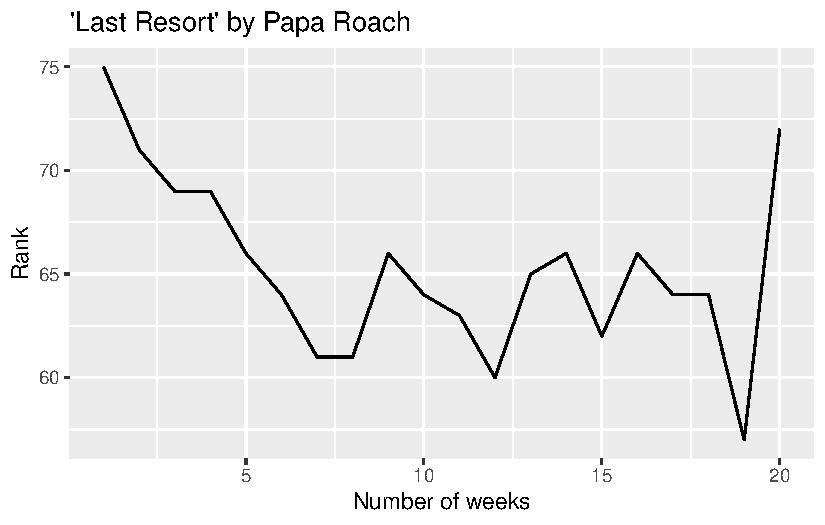
\includegraphics{_descr_stats_DE_files/figure-pdf/unnamed-chunk-16-1.pdf}

}

\end{figure}

\hypertarget{heutige-ziele}{%
\section*{Heutige Ziele}\label{heutige-ziele}}
\addcontentsline{toc}{section}{Heutige Ziele}

Heute werden wir\ldots{}

\begin{itemize}
\tightlist
\item
  die Maße der zentralen Tendenz (wieder) kennenlernen
\item
  Streuungsmaße (neu) kennenlernen
\item
  lernen, wie man die Funktion \texttt{summarise()} von \texttt{dplyr}
  benutzt
\item
  lernen, wie man Zusammenfassungen \texttt{.by} Gruppe erstellt
\end{itemize}

\hypertarget{lust-auf-mehr}{%
\subsection*{Lust auf mehr?}\label{lust-auf-mehr}}
\addcontentsline{toc}{subsection}{Lust auf mehr?}

Ch.4, Section 4.5
\href{https://r4ds.hadley.nz/data-transform.html\#groups}{Groups} in
Wickham et al. (o.~J.)

\hypertarget{einrichtung}{%
\section{Einrichtung}\label{einrichtung}}

\texttt{Session\ \textgreater{}\ Restart\ R} um mit einer neuen Umgebung
zu beginnen.

\begin{Shaded}
\begin{Highlighting}[]
\NormalTok{pacman}\SpecialCharTok{::}\FunctionTok{p\_load}\NormalTok{(tidyverse,}
\NormalTok{               here)}
\end{Highlighting}
\end{Shaded}

\begin{Shaded}
\begin{Highlighting}[]
\NormalTok{df\_flights }\OtherTok{\textless{}{-}} \FunctionTok{read\_csv}\NormalTok{(}\FunctionTok{here}\NormalTok{(}\StringTok{"daten"}\NormalTok{, }\StringTok{"flights.csv"}\NormalTok{))}
\end{Highlighting}
\end{Shaded}

\hypertarget{deskriptive-statistik}{%
\section{Deskriptive Statistik}\label{deskriptive-statistik}}

\begin{itemize}
\item
  Die deskriptive Statistik beschreibt die zentrale Tendenz, die
  Variabilität und die Verteilung der Daten.
\item
  manchmal auch ``zusammenfassende'' Statistik genannt, weil sie die
  beobachteten Daten \emph{zusammenfasst}.
\end{itemize}

\hypertarget{anzahl-der-werte-n}{%
\subsection{\texorpdfstring{Anzahl der Werte
(\(n\))}{Anzahl der Werte (n)}}\label{anzahl-der-werte-n}}

\begin{itemize}
\tightlist
\item
  wichtige Informationen bei der Zusammenfassung von Daten

  \begin{itemize}
  \tightlist
  \item
    Wenn wir mehr Daten haben (höher \(n\)), haben wir mehr Vertrauen in
    die Schlussfolgerungen, die wir aus unseren Daten ziehen, weil wir
    mehr Beweise haben.
  \item
    wird auch zur Berechnung einiger deskriptiver Statistiken verwendet
  \end{itemize}
\end{itemize}

\begin{Shaded}
\begin{Highlighting}[]
\NormalTok{values }\OtherTok{\textless{}{-}} \FunctionTok{c}\NormalTok{(}\DecValTok{3}\NormalTok{,}\DecValTok{1}\NormalTok{,}\DecValTok{2}\NormalTok{)}
\FunctionTok{length}\NormalTok{(values)}
\end{Highlighting}
\end{Shaded}

\begin{verbatim}
[1] 3
\end{verbatim}

\begin{center}\rule{0.5\linewidth}{0.5pt}\end{center}

\begin{tcolorbox}[enhanced jigsaw, breakable, colbacktitle=quarto-callout-note-color!10!white, toptitle=1mm, bottomrule=.15mm, rightrule=.15mm, coltitle=black, toprule=.15mm, opacityback=0, leftrule=.75mm, left=2mm, colframe=quarto-callout-note-color-frame, bottomtitle=1mm, titlerule=0mm, title=\textcolor{quarto-callout-note-color}{\faInfo}\hspace{0.5em}{\texttt{length()} versus \texttt{nrow()} and \texttt{n()}}, arc=.35mm, colback=white, opacitybacktitle=0.6]

\begin{itemize}
\tightlist
\item
  die Funktion ``Länge()'' gibt an, wie viele (horizontale) Werte ein
  Objekt enthält

  \begin{itemize}
  \tightlist
  \item
    Wenn das Objekt ein Datenrahmen ist (statt eines Vektors wie
    ``Werte''), sagt sie uns, wie viele \emph{Spalten} wir haben.
  \end{itemize}
\end{itemize}

\begin{Shaded}
\begin{Highlighting}[]
\FunctionTok{length}\NormalTok{(df\_flights)}
\end{Highlighting}
\end{Shaded}

\begin{verbatim}
[1] 19
\end{verbatim}

\begin{itemize}
\tightlist
\item
  Um die Anzahl der Werte (d.h. Beobachtungen/Zeilen) in einem
  Datenrahmen zu zählen, können wir verwenden

  \begin{itemize}
  \tightlist
  \item
    \texttt{nrow()} (Basis-R-Syntax), oder
  \item
    \texttt{n()} (\texttt{dplyr}-Syntax), das werden wir später noch
    sehen
  \end{itemize}
\end{itemize}

\begin{Shaded}
\begin{Highlighting}[]
\FunctionTok{nrow}\NormalTok{(df\_flights)}
\end{Highlighting}
\end{Shaded}

\begin{verbatim}
[1] 336776
\end{verbatim}

\end{tcolorbox}

\hypertarget{measures-of-central-tendency}{%
\subsection{Measures of central
tendency}\label{measures-of-central-tendency}}

\begin{itemize}
\tightlist
\item
  ziemlich genau das, was wir für \emph{numerische} Variablen mit der
  Funktion \texttt{summary()} erhalten
\end{itemize}

\begin{Shaded}
\begin{Highlighting}[]
\NormalTok{df\_flights }\SpecialCharTok{\%\textgreater{}\%} 
  \FunctionTok{select}\NormalTok{(air\_time, distance) }\SpecialCharTok{\%\textgreater{}\%} 
  \FunctionTok{summary}\NormalTok{() }\SpecialCharTok{\%\textgreater{}\%} 
\NormalTok{  knitr}\SpecialCharTok{::}\FunctionTok{kable}\NormalTok{() }\SpecialCharTok{\%\textgreater{}\%} 
\NormalTok{  kableExtra}\SpecialCharTok{::}\FunctionTok{kable\_styling}\NormalTok{(}\AttributeTok{font\_size =} \DecValTok{30}\NormalTok{)}
\end{Highlighting}
\end{Shaded}

\begin{table}
\centering\begingroup\fontsize{30}{32}\selectfont

\begin{tabular}{l|l|l}
\hline
  &    air\_time &    distance\\
\hline
 & Min.   : 20.0 & Min.   :  17\\
\hline
 & 1st Qu.: 82.0 & 1st Qu.: 502\\
\hline
 & Median :129.0 & Median : 872\\
\hline
 & Mean   :150.7 & Mean   :1040\\
\hline
 & 3rd Qu.:192.0 & 3rd Qu.:1389\\
\hline
 & Max.   :695.0 & Max.   :4983\\
\hline
 & NA's   :9430 & NA\\
\hline
\end{tabular}
\endgroup{}
\end{table}

\hypertarget{durchschnitt-mu}{%
\subsubsection{\texorpdfstring{Durchschnitt
(\(\mu\))}{Durchschnitt (\textbackslash mu)}}\label{durchschnitt-mu}}

\begin{itemize}
\tightlist
\item
  \texttt{mean} = Mittelwert, Durchschnitt
\item
  die Summe aller Werte geteilt durch die Anzahl der Werte
\end{itemize}

\[
\mu = \frac{Summe\;der\;Werte}
           {n}
\]

\begin{center}\rule{0.5\linewidth}{0.5pt}\end{center}

\begin{itemize}
\tightlist
\item
  Wir können den Mittelwert leicht von Hand berechnen, wenn wir nur
  wenige Werte haben
\end{itemize}

\begin{Shaded}
\begin{Highlighting}[]
\NormalTok{(}\DecValTok{3}\SpecialCharTok{+}\DecValTok{1}\SpecialCharTok{+}\DecValTok{2}\NormalTok{)}\SpecialCharTok{/}\DecValTok{3}
\end{Highlighting}
\end{Shaded}

\begin{verbatim}
[1] 2
\end{verbatim}

\begin{itemize}
\tightlist
\item
  wir können die Werte auch als Vektor (eine Liste von Werten derselben
  Klasse) speichern
\item
  und dann die Funktion \texttt{mean()} verwenden, um ihren Mittelwert
  zu berechnen
\end{itemize}

\begin{Shaded}
\begin{Highlighting}[]
\NormalTok{values }\OtherTok{\textless{}{-}} \FunctionTok{c}\NormalTok{(}\DecValTok{3}\NormalTok{,}\DecValTok{1}\NormalTok{,}\DecValTok{2}\NormalTok{)}
\FunctionTok{mean}\NormalTok{(values)}
\end{Highlighting}
\end{Shaded}

\begin{verbatim}
[1] 2
\end{verbatim}

\begin{itemize}
\tightlist
\item
  oder wir können die Funktion \texttt{mean()} auf eine Variable in
  einem Datenrahmen anwenden

  \begin{itemize}
  \tightlist
  \item
    Verwendung des Zeichens \texttt{\$}, um anzugeben, dass eine Spalte
    aus einem Datenrahmen ausgewählt werden soll
  \end{itemize}
\end{itemize}

\begin{Shaded}
\begin{Highlighting}[]
\FunctionTok{mean}\NormalTok{(df\_flights}\SpecialCharTok{$}\NormalTok{distance)}
\end{Highlighting}
\end{Shaded}

\begin{verbatim}
[1] 1039.913
\end{verbatim}

\begin{itemize}
\tightlist
\item
  \texttt{df\_flights\$distance} ist vergleichbar mit
  \texttt{df\_flights\ \%\textgreater{}\%\ select(distance)}
\end{itemize}

\hypertarget{median}{%
\subsubsection{Median}\label{median}}

\begin{itemize}
\tightlist
\item
  \texttt{median} = Median, mediane Wert; der Wert in der Mitte des
  Datensatzes
\item
  Wenn Sie alle Ihre Werte in aufsteigender (oder absteigender)
  Reihenfolge aneinanderreihen, ist der mittlere Wert der Median

  \begin{itemize}
  \tightlist
  \item
    Wenn Sie z. B. 5 Werte haben, ist der 3. Wert der Median
  \item
    bei 6 Werten ist der Mittelwert aus dem 3. und 4. Wert der Median
  \end{itemize}
\item
  50\% der Daten liegen unter diesem Wert, 50\% darüber
\end{itemize}

\begin{Shaded}
\begin{Highlighting}[]
\FunctionTok{median}\NormalTok{(df\_flights}\SpecialCharTok{$}\NormalTok{distance)}
\end{Highlighting}
\end{Shaded}

\begin{verbatim}
[1] 872
\end{verbatim}

\hypertarget{modalwert}{%
\subsubsection{Modalwert}\label{modalwert}}

\begin{itemize}
\tightlist
\item
  \texttt{mode} = Modalwert; der Wert, der am häufigsten in einem
  Datensatz vorkommt
\item
  Es gibt keine R-Funktion zur Bestimmung des ``Modus'', aber wir können
  ihn mit einem Histogramm visualisieren
\end{itemize}

\begin{Shaded}
\begin{Highlighting}[]
\NormalTok{df\_flights }\SpecialCharTok{\%\textgreater{}\%} 
  \FunctionTok{ggplot}\NormalTok{(}\FunctionTok{aes}\NormalTok{(}\AttributeTok{x =}\NormalTok{ distance)) }\SpecialCharTok{+}
  \FunctionTok{geom\_histogram}\NormalTok{() }\SpecialCharTok{+}
  \FunctionTok{theme\_minimal}\NormalTok{() }
\end{Highlighting}
\end{Shaded}

\begin{figure}[H]

{\centering 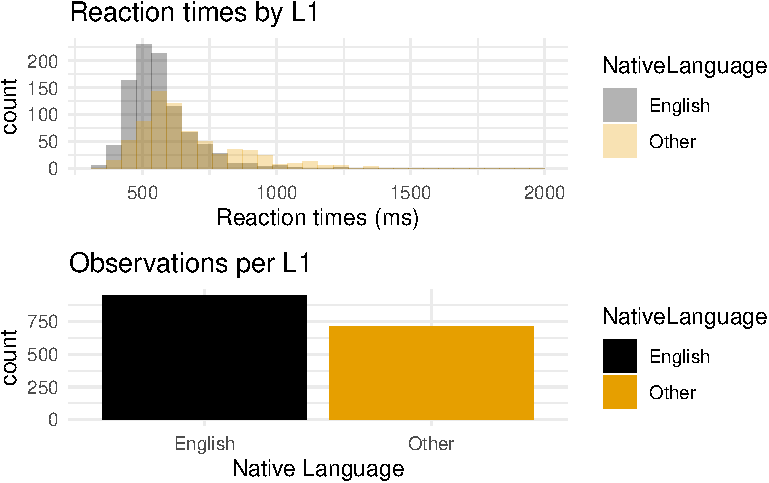
\includegraphics{_descr_stats_DE_files/figure-pdf/unnamed-chunk-27-1.pdf}

}

\end{figure}

\hypertarget{mauxdfe-der-streuung}{%
\subsection{Maße der Streuung}\label{mauxdfe-der-streuung}}

\begin{itemize}
\tightlist
\item
  Maße der zentralen Tendenz beschreiben die Mitte der Daten
  (normalerweise)
\item
  Streuungsmaße beschreiben die Verteilung der Datenpunkte
\end{itemize}

\hypertarget{wertebereich}{%
\subsubsection{Wertebereich}\label{wertebereich}}

\begin{itemize}
\tightlist
\item
  \texttt{range} = Wertebereich

  \begin{itemize}
  \tightlist
  \item
    kann sich auf den höchsten und den niedrigsten Wert beziehen, oder
  \item
    die Differenz zwischen höchstem und niedrigstem Wert
  \end{itemize}
\end{itemize}

\begin{center}\rule{0.5\linewidth}{0.5pt}\end{center}

\begin{itemize}
\tightlist
\item
  \texttt{max()} und \texttt{min()} den höchsten und den niedrigsten
  Wert ausdrucken
\end{itemize}

\begin{Shaded}
\begin{Highlighting}[]
\FunctionTok{max}\NormalTok{(values)}
\end{Highlighting}
\end{Shaded}

\begin{verbatim}
[1] 3
\end{verbatim}

\begin{Shaded}
\begin{Highlighting}[]
\FunctionTok{min}\NormalTok{(values)}
\end{Highlighting}
\end{Shaded}

\begin{verbatim}
[1] 1
\end{verbatim}

\begin{itemize}
\tightlist
\item
  \texttt{range()} druckt den niedrigsten und den höchsten Wert
\end{itemize}

\begin{Shaded}
\begin{Highlighting}[]
\FunctionTok{range}\NormalTok{(values)}
\end{Highlighting}
\end{Shaded}

\begin{verbatim}
[1] 1 3
\end{verbatim}

\begin{itemize}
\tightlist
\item
  können wir die Differenz zwischen diesen Werten berechnen:
\end{itemize}

\begin{Shaded}
\begin{Highlighting}[]
\FunctionTok{max}\NormalTok{(values) }\SpecialCharTok{{-}} \FunctionTok{min}\NormalTok{(values)}
\end{Highlighting}
\end{Shaded}

\begin{verbatim}
[1] 2
\end{verbatim}

\hypertarget{standardabweichung-sd-or-sigma}{%
\subsubsection{\texorpdfstring{Standardabweichung (\texttt{sd} or
\(\sigma\))}{Standardabweichung (sd or \textbackslash sigma)}}\label{standardabweichung-sd-or-sigma}}

\begin{itemize}
\item
  ein Maß dafür, wie gestreut die Daten \emph{im Verhältnis zum
  Mittelwert} sind

  \begin{itemize}
  \tightlist
  \item
    eine niedrige Standardabweichung bedeutet, dass die Daten um den
    Mittelwert herum gruppiert sind (d.~h. es gibt eine geringere
    Streuung)
  \item
    eine hohe Standardabweichung bedeutet, dass die Daten stärker
    gestreut sind
  \end{itemize}
\item
  Die Standardabweichung wird sehr oft angegeben, wenn der Mittelwert
  angegeben wird.
\item
  um \texttt{sd} zu berechnen

  \begin{itemize}
  \tightlist
  \item
    die Quadratwurzel (\(\sqrt{}\)) der Summe der quadrierten
    Wertabweichungen vom Mittelwert (\((x - \mu)^2\)) geteilt durch die
    Anzahl der Beobachtungen minus 1 (\(n-1\))
  \end{itemize}
\end{itemize}

\begin{Shaded}
\begin{Highlighting}[]
\FunctionTok{sd}\NormalTok{(values)}
\end{Highlighting}
\end{Shaded}

\begin{verbatim}
[1] 1
\end{verbatim}

\begin{center}\rule{0.5\linewidth}{0.5pt}\end{center}

\begin{itemize}
\tightlist
\item
  unsere Werte (\(x\)) sind:
\end{itemize}

\begin{Shaded}
\begin{Highlighting}[]
\NormalTok{values}
\end{Highlighting}
\end{Shaded}

\begin{verbatim}
[1] 3 1 2
\end{verbatim}

\begin{itemize}
\tightlist
\item
  der Mittelwert (\(\mu\)) ist:
\end{itemize}

\begin{Shaded}
\begin{Highlighting}[]
\FunctionTok{mean}\NormalTok{(values)}
\end{Highlighting}
\end{Shaded}

\begin{verbatim}
[1] 2
\end{verbatim}

\begin{itemize}
\tightlist
\item
  die Anzahl der Werte (\(n\)) ist:
\end{itemize}

\begin{Shaded}
\begin{Highlighting}[]
\FunctionTok{length}\NormalTok{(values)}
\end{Highlighting}
\end{Shaded}

\begin{verbatim}
[1] 3
\end{verbatim}

\begin{itemize}
\tightlist
\item
  die Standardabweichung (\(\sigma\)) ist:
\end{itemize}

\begin{Shaded}
\begin{Highlighting}[]
\FunctionTok{sd}\NormalTok{(values)}
\end{Highlighting}
\end{Shaded}

\begin{verbatim}
[1] 1
\end{verbatim}

\begin{align}

\sigma & = \sqrt{\frac{(x_1-\mu)^2 + (x_2-\mu)^2 + (x_3-\mu)^2}{N-1}}
\\
& = \sqrt{\frac{(3-\mu)^2 + (1-\mu)^2 + (2-\mu)^2}{N-1}}
\\
& = \sqrt{\frac{(3-2)^2 + (1-2)^2 + (2-2)^2}{3-1}}
\\
& = \sqrt{\frac{(1)^2 + (-1)^2 + (0)^2}{2}}
\\
& = \sqrt{\frac{1 + 1 + 0}{2}}
\\
& = \sqrt{\frac{2}{2}} = \sqrt{1} = 1

\end{align}

\begin{center}\rule{0.5\linewidth}{0.5pt}\end{center}

\begin{itemize}
\tightlist
\item
  Inwiefern ist die Standardabweichung hilfreich?

  \begin{itemize}
  \tightlist
  \item
    Sie gibt uns ein Maß dafür, wie ``eng'' die beobachteten Werte am
    Mittelwert liegen.
  \end{itemize}
\item
  Verschiedene Datensätze können zum Beispiel denselben Mittelwert
  haben:
\end{itemize}

\begin{Shaded}
\begin{Highlighting}[]
\NormalTok{values2 }\OtherTok{\textless{}{-}} \FunctionTok{c}\NormalTok{(}\DecValTok{55}\NormalTok{,}\DecValTok{55}\NormalTok{,}\DecValTok{55}\NormalTok{,}\DecValTok{55}\NormalTok{,}\DecValTok{55}\NormalTok{,}\DecValTok{57}\NormalTok{,}\DecValTok{57}\NormalTok{,}\DecValTok{57}\NormalTok{,}\DecValTok{57}\NormalTok{,}\DecValTok{57}\NormalTok{)}
\NormalTok{values3 }\OtherTok{\textless{}{-}} \FunctionTok{c}\NormalTok{(}\DecValTok{1}\NormalTok{,}\DecValTok{1}\NormalTok{,}\DecValTok{1}\NormalTok{,}\DecValTok{1}\NormalTok{,}\DecValTok{100}\NormalTok{,}\DecValTok{100}\NormalTok{,}\DecValTok{100}\NormalTok{,}\DecValTok{100}\NormalTok{,}\DecValTok{100}\NormalTok{)}
\end{Highlighting}
\end{Shaded}

\begin{Shaded}
\begin{Highlighting}[]
\FunctionTok{mean}\NormalTok{(values2)}
\end{Highlighting}
\end{Shaded}

\begin{verbatim}
[1] 56
\end{verbatim}

\begin{Shaded}
\begin{Highlighting}[]
\FunctionTok{mean}\NormalTok{(values3)}
\end{Highlighting}
\end{Shaded}

\begin{verbatim}
[1] 56
\end{verbatim}

\begin{itemize}
\tightlist
\item
  \texttt{values2} und \texttt{values3} haben den gleichen Mittelwert

  \begin{itemize}
  \tightlist
  \item
    Wenn wir nur den Mittelwert berechnen würden, könnten wir zu dem
    Schluss kommen, dass die Daten ähnlich sind.
  \end{itemize}
\item
  aber ihre Standardabweichungen werden sich unterscheiden, weil die
  beobachteten Werte alle unterschiedlich weit vom Mittelwert abweichen
\item
  Welcher Vektor wird Ihrer Meinung nach die \emph{geringste}
  Standardabweichung haben? Und warum?
\end{itemize}

\begin{Shaded}
\begin{Highlighting}[]
\FunctionTok{sd}\NormalTok{(values2)}
\end{Highlighting}
\end{Shaded}

\begin{verbatim}
[1] 1.054093
\end{verbatim}

\begin{Shaded}
\begin{Highlighting}[]
\FunctionTok{sd}\NormalTok{(values3)}
\end{Highlighting}
\end{Shaded}

\begin{verbatim}
[1] 52.17758
\end{verbatim}

\begin{center}\rule{0.5\linewidth}{0.5pt}\end{center}

\begin{tcolorbox}[enhanced jigsaw, breakable, colbacktitle=quarto-callout-note-color!10!white, toptitle=1mm, bottomrule=.15mm, rightrule=.15mm, coltitle=black, toprule=.15mm, opacityback=0, leftrule=.75mm, left=2mm, colframe=quarto-callout-note-color-frame, bottomtitle=1mm, titlerule=0mm, title=\textcolor{quarto-callout-note-color}{\faInfo}\hspace{0.5em}{CBerechnung der Standardabweichung}, arc=.35mm, colback=white, opacitybacktitle=0.6]

\begin{itemize}
\tightlist
\item
  Berechnen Sie zunächst die Abweichung jedes Wertes vom Mittelwert

  \begin{itemize}
  \tightlist
  \item
    und quadriere diesen Wert
  \end{itemize}
\item
  addiere alle diese quadrierten Abweichungswerte

  \begin{itemize}
  \tightlist
  \item
    dividiere durch die Anzahl der Beobachtungen \emph{bis auf eine}
    (\(n-1\))
  \end{itemize}
\item
  dies ist nun die \emph{Varianz}, um die Standardabweichung der
  Population zu erhalten, berechnet man die Quadratwurzel dieses Wertes
\end{itemize}

\begin{align}

\sigma & = \sqrt\frac{(56-1)^2 + (56-1)^2 + (56-1)^2 + (56-1)^2 + (56-100)^2 +
        (56-100)^2 + (56-100)^2 + (56-100)^2 + (56-100)^2 + (56-100)^2}{n-1}
\\
& = \sqrt{\frac{3025 + 3025 + 3025 + 3025 + 1936 + 1936 + 1936 + 1936 + 1936}{9-1}}
\\
& = \sqrt{\frac{21780}{8}}
\\
& = \sqrt{2722.5}
\\
& = 52.17758

\end{align}

\begin{itemize}
\item
  Da wir durch die Anzahl der Beobachtungen (minus 1) dividieren, wird
  die Standardabweichung kleiner sein, wenn wir \emph{mehr}
  Beobachtungen haben (und daher durch eine größere Zahl dividieren)
  (denn wenn wir durch eine große Zahl dividieren, ist das Produkt viel
  kleiner)
\item
  Beispiel: Wenn wir 100 durch die Zahl 2 teilen, ist das Ergebnis 50.
  Wenn wir 100 durch eine größere Zahl, wie 50, teilen, ist das Ergebnis
  (2) kleiner.
\end{itemize}

\end{tcolorbox}

\hypertarget{dplyrsummarise}{%
\section{\texorpdfstring{\texttt{dplyr::summarise}}{dplyr::summarise}}\label{dplyrsummarise}}

\begin{itemize}
\tightlist
\item
  berechnet Zusammenfassungen von Daten

  \begin{itemize}
  \tightlist
  \item
    aber wir müssen ihm sagen, \emph{was} es berechnen soll und für
    welche Variable(n)
  \end{itemize}
\end{itemize}

\begin{Shaded}
\begin{Highlighting}[]
\NormalTok{df\_flights }\SpecialCharTok{\%\textgreater{}\%} 
  \FunctionTok{summarise}\NormalTok{(}\AttributeTok{N =} \FunctionTok{n}\NormalTok{())}
\end{Highlighting}
\end{Shaded}

\begin{verbatim}
# A tibble: 1 x 1
       N
   <int>
1 336776
\end{verbatim}

\begin{center}\rule{0.5\linewidth}{0.5pt}\end{center}

\begin{itemize}
\tightlist
\item
  wir können auch mehrere Berechnungen auf einmal durchführen
\end{itemize}

\begin{Shaded}
\begin{Highlighting}[]
\NormalTok{df\_flights }\SpecialCharTok{\%\textgreater{}\%} 
  \FunctionTok{summarise}\NormalTok{(}\AttributeTok{mean\_distance =} \FunctionTok{mean}\NormalTok{(distance, }\AttributeTok{na.rm=}\NormalTok{T),}
            \AttributeTok{sd\_distance =} \FunctionTok{sd}\NormalTok{(distance, }\AttributeTok{na.rm =}\NormalTok{ T),}
            \AttributeTok{N =} \FunctionTok{n}\NormalTok{()) }\SpecialCharTok{\%\textgreater{}\%} 
\NormalTok{  knitr}\SpecialCharTok{::}\FunctionTok{kable}\NormalTok{() }\SpecialCharTok{\%\textgreater{}\%} 
\NormalTok{  kableExtra}\SpecialCharTok{::}\FunctionTok{kable\_styling}\NormalTok{()}
\end{Highlighting}
\end{Shaded}

\begin{table}
\centering
\begin{tabular}{r|r|r}
\hline
mean\_distance & sd\_distance & N\\
\hline
1039.913 & 733.233 & 336776\\
\hline
\end{tabular}
\end{table}

\begin{center}\rule{0.5\linewidth}{0.5pt}\end{center}

\begin{itemize}
\tightlist
\item
  und wir können Berechnungen angeben
\end{itemize}

\begin{Shaded}
\begin{Highlighting}[]
\NormalTok{df\_flights }\SpecialCharTok{\%\textgreater{}\%} 
  \FunctionTok{summarise}\NormalTok{(}\AttributeTok{range\_distance =} \FunctionTok{max}\NormalTok{(distance) }\SpecialCharTok{{-}} \FunctionTok{min}\NormalTok{(distance))}
\end{Highlighting}
\end{Shaded}

\begin{verbatim}
# A tibble: 1 x 1
  range_distance
           <dbl>
1           4966
\end{verbatim}

\hypertarget{fehlende-werte}{%
\subsection{Fehlende Werte}\label{fehlende-werte}}

\begin{itemize}
\tightlist
\item
  einige Berechnungen sind bei fehlenden Werten nicht möglich

  \begin{itemize}
  \tightlist
  \item
    die Variable ``air\_time'' hat einige fehlende Werte
  \end{itemize}
\end{itemize}

\begin{Shaded}
\begin{Highlighting}[]
\NormalTok{df\_flights }\SpecialCharTok{\%\textgreater{}\%} 
  \FunctionTok{select}\NormalTok{(air\_time, distance) }\SpecialCharTok{\%\textgreater{}\%} 
  \FunctionTok{summary}\NormalTok{()}
\end{Highlighting}
\end{Shaded}

\begin{verbatim}
    air_time        distance   
 Min.   : 20.0   Min.   :  17  
 1st Qu.: 82.0   1st Qu.: 502  
 Median :129.0   Median : 872  
 Mean   :150.7   Mean   :1040  
 3rd Qu.:192.0   3rd Qu.:1389  
 Max.   :695.0   Max.   :4983  
 NA's   :9430                  
\end{verbatim}

\begin{Shaded}
\begin{Highlighting}[]
\NormalTok{df\_flights }\SpecialCharTok{\%\textgreater{}\%} 
  \FunctionTok{summarise}\NormalTok{(}\AttributeTok{mean\_air\_time =} \FunctionTok{mean}\NormalTok{(air\_time))}
\end{Highlighting}
\end{Shaded}

\begin{verbatim}
# A tibble: 1 x 1
  mean_air_time
          <dbl>
1            NA
\end{verbatim}

\begin{center}\rule{0.5\linewidth}{0.5pt}\end{center}

\begin{itemize}
\tightlist
\item
  Bei der Arbeit mit realen Daten ist es nicht trivial, wie man mit
  fehlenden Werten umgeht.

  \begin{itemize}
  \tightlist
  \item
    z.B. könnten wir alle ``N''-Werte in ``0'' umwandeln, wenn wir
    wollen, dass sie zur Berechnung des ``Mittelwerts'' beitragen
  \item
    aber in den meisten Fällen wollen wir sie einfach entfernen (wie wir
    es schon oft getan haben)
  \end{itemize}
\item
  Wir können dies leicht mit dem \texttt{dplyr}-Verb \texttt{drop\_na()}
  tun
\end{itemize}

\begin{Shaded}
\begin{Highlighting}[]
\NormalTok{df\_flights }\SpecialCharTok{\%\textgreater{}\%} 
  \FunctionTok{drop\_na}\NormalTok{() }\SpecialCharTok{\%\textgreater{}\%} 
  \FunctionTok{summarise}\NormalTok{(}\AttributeTok{mean =} \FunctionTok{mean}\NormalTok{(air\_time))}
\end{Highlighting}
\end{Shaded}

\begin{verbatim}
# A tibble: 1 x 1
   mean
  <dbl>
1  151.
\end{verbatim}

\hypertarget{gruppierung-von-variablen}{%
\section{Gruppierung von Variablen}\label{gruppierung-von-variablen}}

\begin{itemize}
\tightlist
\item
  Wir wollen nicht immer nur die zusammenfassenden Statistiken für einen
  gesamten Datensatz kennen, aber

  \begin{itemize}
  \tightlist
  \item
    Wir wollen in der Regel bestimmte Gruppen \emph{vergleichen} (z. B.
    den Vergleich von ``Flugzeit'' zwischen Fluggesellschaften).
  \end{itemize}
\end{itemize}

\hypertarget{by}{%
\subsection{\texorpdfstring{\texttt{.by\ =}}{.by =}}\label{by}}

\begin{itemize}
\tightlist
\item
  das brandneue Argument \texttt{.by\ =} in \texttt{summarise()}
  berechnet unsere Berechnungen auf gruppierten Teilmengen der Daten
  (erst ein paar Monate alt!)

  \begin{itemize}
  \tightlist
  \item
    Es nimmt eine ``Variable'' (d.h. einen Spaltennamen) und gruppiert
    nach den Ebenen dieser Variable
  \end{itemize}
\end{itemize}

\begin{center}\rule{0.5\linewidth}{0.5pt}\end{center}

\begin{Shaded}
\begin{Highlighting}[]
\NormalTok{df\_flights }\SpecialCharTok{\%\textgreater{}\%} 
  \FunctionTok{drop\_na}\NormalTok{() }\SpecialCharTok{\%\textgreater{}\%} 
  \FunctionTok{summarise}\NormalTok{(}\AttributeTok{mean\_air\_time =} \FunctionTok{mean}\NormalTok{(air\_time),}
            \AttributeTok{mean\_distance =} \FunctionTok{mean}\NormalTok{(distance),}
            \AttributeTok{N =} \FunctionTok{n}\NormalTok{(),}
            \AttributeTok{.by =}\NormalTok{ month) }\SpecialCharTok{\%\textgreater{}\%} 
  \FunctionTok{arrange}\NormalTok{(mean\_air\_time)}
\end{Highlighting}
\end{Shaded}

\begin{verbatim}
# A tibble: 12 x 4
   month mean_air_time mean_distance     N
   <dbl>         <dbl>         <dbl> <int>
 1     9          143.         1049. 27010
 2     5          146.         1049. 28128
 3     7          147.         1070. 28293
 4     8          148.         1069. 28756
 5    10          149.         1042. 28618
 6     3          149.         1023. 27902
 7     6          150.         1074. 27075
 8     2          151.         1008. 23611
 9     4          153.         1048. 27564
10     1          154.         1014. 26398
11    11          155.         1052. 26971
12    12          163.         1076. 27020
\end{verbatim}

\hypertarget{gruppieren-nach-mehreren-variablen}{%
\subsection{Gruppieren nach mehreren
Variablen}\label{gruppieren-nach-mehreren-variablen}}

\begin{itemize}
\tightlist
\item
  Wir können auch nach mehreren Variablen gruppieren

  \begin{itemize}
  \tightlist
  \item
    Dazu benötigen wir \texttt{concatenate} (\texttt{c()})
  \end{itemize}
\item
  wir filtern, um nur ein paar Träger zu haben, damit unsere Ausgabe
  nicht zu lang wird
\end{itemize}

\begin{center}\rule{0.5\linewidth}{0.5pt}\end{center}

\begin{Shaded}
\begin{Highlighting}[numbers=left,,]
\NormalTok{df\_flights }\SpecialCharTok{\%\textgreater{}\%} 
  \FunctionTok{drop\_na}\NormalTok{() }\SpecialCharTok{\%\textgreater{}\%}
  \FunctionTok{filter}\NormalTok{(carrier }\SpecialCharTok{\%in\%} \FunctionTok{c}\NormalTok{(}\StringTok{"UA"}\NormalTok{, }\StringTok{"AA"}\NormalTok{)) }\SpecialCharTok{\%\textgreater{}\%} 
  \FunctionTok{summarise}\NormalTok{(}\AttributeTok{mean\_air\_time =} \FunctionTok{mean}\NormalTok{(air\_time),}
            \AttributeTok{mean\_distance =} \FunctionTok{mean}\NormalTok{(distance),}
            \AttributeTok{N =} \FunctionTok{n}\NormalTok{(),}
            \AttributeTok{.by =} \FunctionTok{c}\NormalTok{(month, carrier)) }\SpecialCharTok{\%\textgreater{}\%} 
  \FunctionTok{arrange}\NormalTok{(month, carrier) }\SpecialCharTok{\%\textgreater{}\%} 
\NormalTok{  knitr}\SpecialCharTok{::}\FunctionTok{kable}\NormalTok{() }\SpecialCharTok{\%\textgreater{}\%} 
\NormalTok{  kableExtra}\SpecialCharTok{::}\FunctionTok{kable\_styling}\NormalTok{(}\AttributeTok{font\_size =} \DecValTok{20}\NormalTok{)}
\end{Highlighting}
\end{Shaded}

\begin{table}
\centering\begingroup\fontsize{20}{22}\selectfont

\begin{tabular}{r|l|r|r|r}
\hline
month & carrier & mean\_air\_time & mean\_distance & N\\
\hline
1 & AA & 199.5433 & 1353.099 & 2724\\
\hline
1 & UA & 213.7022 & 1463.894 & 4590\\
\hline
2 & AA & 197.9195 & 1352.686 & 2399\\
\hline
2 & UA & 207.4393 & 1437.190 & 4157\\
\hline
3 & AA & 192.3532 & 1349.525 & 2741\\
\hline
3 & UA & 204.7959 & 1454.933 & 4909\\
\hline
4 & AA & 192.9615 & 1343.950 & 2649\\
\hline
4 & UA & 212.0633 & 1504.828 & 4978\\
\hline
5 & AA & 183.4554 & 1341.822 & 2749\\
\hline
5 & UA & 209.1620 & 1559.828 & 4890\\
\hline
6 & AA & 183.4868 & 1338.606 & 2683\\
\hline
6 & UA & 213.0440 & 1580.517 & 4885\\
\hline
7 & AA & 178.3669 & 1328.671 & 2769\\
\hline
7 & UA & 207.8638 & 1581.408 & 4971\\
\hline
8 & AA & 179.4030 & 1326.186 & 2819\\
\hline
8 & UA & 212.0912 & 1593.323 & 5085\\
\hline
9 & AA & 179.3695 & 1344.793 & 2568\\
\hline
9 & UA & 208.0990 & 1571.911 & 4636\\
\hline
10 & AA & 186.8477 & 1337.230 & 2699\\
\hline
10 & UA & 210.3654 & 1528.576 & 5035\\
\hline
11 & AA & 193.3208 & 1344.323 & 2550\\
\hline
11 & UA & 218.2343 & 1534.453 & 4827\\
\hline
12 & AA & 200.7724 & 1361.288 & 2597\\
\hline
12 & UA & 224.2924 & 1546.725 & 4819\\
\hline
\end{tabular}
\endgroup{}
\end{table}

\begin{center}\rule{0.5\linewidth}{0.5pt}\end{center}

\begin{tcolorbox}[enhanced jigsaw, breakable, colbacktitle=quarto-callout-note-color!10!white, toptitle=1mm, bottomrule=.15mm, rightrule=.15mm, coltitle=black, toprule=.15mm, opacityback=0, leftrule=.75mm, left=2mm, colframe=quarto-callout-note-color-frame, bottomtitle=1mm, titlerule=0mm, title=\textcolor{quarto-callout-note-color}{\faInfo}\hspace{0.5em}{\texttt{group\_by()}}, arc=.35mm, colback=white, opacitybacktitle=0.6]

\begin{itemize}
\tightlist
\item
  vor \texttt{.by()} haben wir das \texttt{dplyr}-Verb
  \texttt{group\_by()} und \texttt{ungroup()} verwendet

  \begin{itemize}
  \tightlist
  \item
    Ich bevorzuge das neue \texttt{.by}, weil es die Gruppierung lokal
    hält (keine Notwendigkeit für \texttt{ungroup()})
  \item
    Behalten Sie dies im Hinterkopf, Sie könnten \texttt{group\_by()} in
    freier Wildbahn sehen
  \end{itemize}
\end{itemize}

\begin{Shaded}
\begin{Highlighting}[numbers=left,,]
\NormalTok{df\_flights }\SpecialCharTok{\%\textgreater{}\%} 
  \FunctionTok{drop\_na}\NormalTok{() }\SpecialCharTok{\%\textgreater{}\%}
  \FunctionTok{filter}\NormalTok{(carrier }\SpecialCharTok{\%in\%} \FunctionTok{c}\NormalTok{(}\StringTok{"UA"}\NormalTok{, }\StringTok{"AA"}\NormalTok{)) }\SpecialCharTok{\%\textgreater{}\%} 
  \FunctionTok{group\_by}\NormalTok{(month, carrier) }\SpecialCharTok{\%\textgreater{}\%} 
  \FunctionTok{summarise}\NormalTok{(}\AttributeTok{mean\_air\_time =} \FunctionTok{mean}\NormalTok{(air\_time),}
            \AttributeTok{mean\_distance =} \FunctionTok{mean}\NormalTok{(distance),}
            \AttributeTok{N =} \FunctionTok{n}\NormalTok{()) }\SpecialCharTok{\%\textgreater{}\%} 
  \FunctionTok{ungroup}\NormalTok{() }\SpecialCharTok{\%\textgreater{}\%} 
  \FunctionTok{arrange}\NormalTok{(month, carrier) }\SpecialCharTok{\%\textgreater{}\%} 
  \FunctionTok{head}\NormalTok{(}\AttributeTok{n =} \DecValTok{10}\NormalTok{) }\SpecialCharTok{\%\textgreater{}\%} 
\NormalTok{  knitr}\SpecialCharTok{::}\FunctionTok{kable}\NormalTok{() }\SpecialCharTok{\%\textgreater{}\%} 
\NormalTok{  kableExtra}\SpecialCharTok{::}\FunctionTok{kable\_styling}\NormalTok{(}\AttributeTok{font\_size =} \DecValTok{20}\NormalTok{) }
\end{Highlighting}
\end{Shaded}

\begin{table}
\centering\begingroup\fontsize{20}{22}\selectfont

\begin{tabular}{r|l|r|r|r}
\hline
month & carrier & mean\_air\_time & mean\_distance & N\\
\hline
1 & AA & 199.5433 & 1353.099 & 2724\\
\hline
1 & UA & 213.7022 & 1463.894 & 4590\\
\hline
2 & AA & 197.9195 & 1352.686 & 2399\\
\hline
2 & UA & 207.4393 & 1437.190 & 4157\\
\hline
3 & AA & 192.3532 & 1349.525 & 2741\\
\hline
3 & UA & 204.7959 & 1454.933 & 4909\\
\hline
4 & AA & 192.9615 & 1343.950 & 2649\\
\hline
4 & UA & 212.0633 & 1504.828 & 4978\\
\hline
5 & AA & 183.4554 & 1341.822 & 2749\\
\hline
5 & UA & 209.1620 & 1559.828 & 4890\\
\hline
\end{tabular}
\endgroup{}
\end{table}

\end{tcolorbox}

\hypertarget{anscombes-quartet}{%
\section{Anscombe's Quartet}\label{anscombes-quartet}}

\begin{itemize}
\tightlist
\item
  Francis Anscombe erstellte 1973 4 Datensätze, um zu zeigen, wie
  wichtig es ist, Daten zu visualisieren, bevor man sie analysiert und
  ein Modell erstellt

  \begin{itemize}
  \tightlist
  \item
    Diese vier Diagramme stellen 4 Datensätze dar, die alle einen nahezu
    identischen Mittelwert und eine Standardabweichung, aber sehr
    unterschiedliche Verteilungen aufweisen
  \end{itemize}
\end{itemize}

\hypertarget{tbl-anscombe}{}
\begin{table}
\caption{\label{tbl-anscombe}Summary stats of Anscombe's quratet datasets }\tabularnewline

\centering\begingroup\fontsize{20}{22}\selectfont

\begin{tabular}{l|r|r|r|r|r|r|r}
\hline
grp & mean\_x & mean\_y & min\_x & min\_y & max\_x & max\_y & crrltn\\
\hline
Group 1 & 9 & 7.500909 & 4 & 4.26 & 14 & 10.84 & 0.8164205\\
\hline
Group 2 & 9 & 7.500909 & 4 & 3.10 & 14 & 9.26 & 0.8162365\\
\hline
Group 3 & 9 & 7.500000 & 4 & 5.39 & 14 & 12.74 & 0.8162867\\
\hline
Group 4 & 9 & 7.500909 & 8 & 5.25 & 19 & 12.50 & 0.8165214\\
\hline
\end{tabular}
\endgroup{}
\end{table}

\begin{center}\rule{0.5\linewidth}{0.5pt}\end{center}

\begin{figure}

{\centering 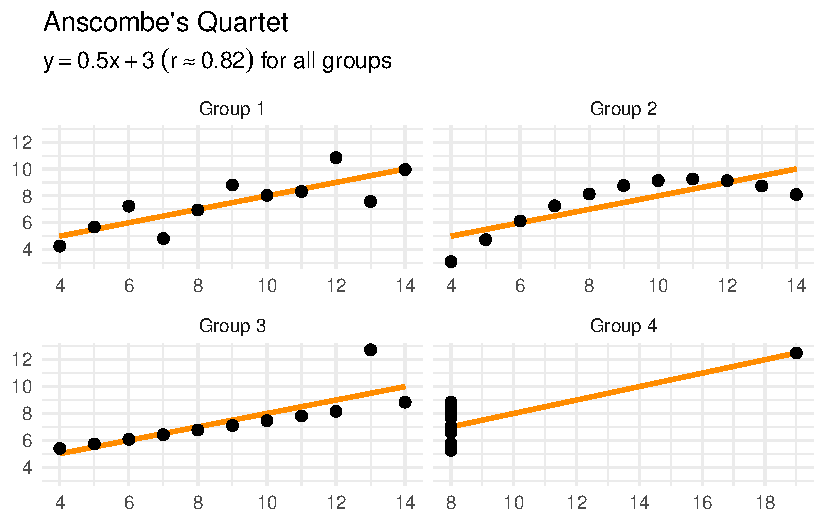
\includegraphics{_descr_stats_DE_files/figure-pdf/fig-anscombe-1.pdf}

}

\caption{\label{fig-anscombe}Plots of Anscombe's quratet distributions}

\end{figure}

\hypertarget{datasaurrus}{%
\subsection{DatasaurRus}\label{datasaurrus}}

\begin{itemize}
\tightlist
\item
  das Paket \texttt{datasaurRus} enthält einige weitere Datensätze, die
  ähnliche Mittelwerte und SD, aber unterschiedliche Verteilungen
  aufweisen
\end{itemize}

\begin{Shaded}
\begin{Highlighting}[]
\NormalTok{pacman}\SpecialCharTok{::}\FunctionTok{p\_load}\NormalTok{(}\StringTok{"datasauRus"}\NormalTok{)}
\end{Highlighting}
\end{Shaded}

\begin{Shaded}
\begin{Highlighting}[]
\NormalTok{datasaurus\_dozen }\SpecialCharTok{\%\textgreater{}\%} 
    \FunctionTok{group\_by}\NormalTok{(dataset) }\SpecialCharTok{\%\textgreater{}\%} 
    \FunctionTok{summarize}\NormalTok{(}
      \AttributeTok{mean\_x    =} \FunctionTok{mean}\NormalTok{(x),}
      \AttributeTok{mean\_y    =} \FunctionTok{mean}\NormalTok{(y),}
      \AttributeTok{std\_dev\_x =} \FunctionTok{sd}\NormalTok{(x),}
      \AttributeTok{std\_dev\_y =} \FunctionTok{sd}\NormalTok{(y),}
      \AttributeTok{corr\_x\_y  =} \FunctionTok{cor}\NormalTok{(x, y)}
\NormalTok{    ) }\SpecialCharTok{\%\textgreater{}\%} 
\NormalTok{  knitr}\SpecialCharTok{::}\FunctionTok{kable}\NormalTok{() }\SpecialCharTok{\%\textgreater{}\%} 
\NormalTok{  kableExtra}\SpecialCharTok{::}\FunctionTok{kable\_styling}\NormalTok{(}\AttributeTok{font\_size =} \DecValTok{20}\NormalTok{)}
\end{Highlighting}
\end{Shaded}

\hypertarget{tbl-datasauRus}{}
\begin{table}
\caption{\label{tbl-datasauRus}Summary stats of datasauRus datasets }\tabularnewline

\centering\begingroup\fontsize{20}{22}\selectfont

\begin{tabular}{l|r|r|r|r|r}
\hline
dataset & mean\_x & mean\_y & std\_dev\_x & std\_dev\_y & corr\_x\_y\\
\hline
away & 54.26610 & 47.83472 & 16.76983 & 26.93974 & -0.0641284\\
\hline
bullseye & 54.26873 & 47.83082 & 16.76924 & 26.93573 & -0.0685864\\
\hline
circle & 54.26732 & 47.83772 & 16.76001 & 26.93004 & -0.0683434\\
\hline
dino & 54.26327 & 47.83225 & 16.76514 & 26.93540 & -0.0644719\\
\hline
dots & 54.26030 & 47.83983 & 16.76774 & 26.93019 & -0.0603414\\
\hline
h\_lines & 54.26144 & 47.83025 & 16.76590 & 26.93988 & -0.0617148\\
\hline
high\_lines & 54.26881 & 47.83545 & 16.76670 & 26.94000 & -0.0685042\\
\hline
slant\_down & 54.26785 & 47.83590 & 16.76676 & 26.93610 & -0.0689797\\
\hline
slant\_up & 54.26588 & 47.83150 & 16.76885 & 26.93861 & -0.0686092\\
\hline
star & 54.26734 & 47.83955 & 16.76896 & 26.93027 & -0.0629611\\
\hline
v\_lines & 54.26993 & 47.83699 & 16.76996 & 26.93768 & -0.0694456\\
\hline
wide\_lines & 54.26692 & 47.83160 & 16.77000 & 26.93790 & -0.0665752\\
\hline
x\_shape & 54.26015 & 47.83972 & 16.76996 & 26.93000 & -0.0655833\\
\hline
\end{tabular}
\endgroup{}
\end{table}

\begin{center}\rule{0.5\linewidth}{0.5pt}\end{center}

\begin{itemize}
\tightlist
\item
  Wenn wir die Datensätze grafisch darstellen, sehen sie alle sehr
  unterschiedlich aus!
\end{itemize}

\begin{figure}

{\centering 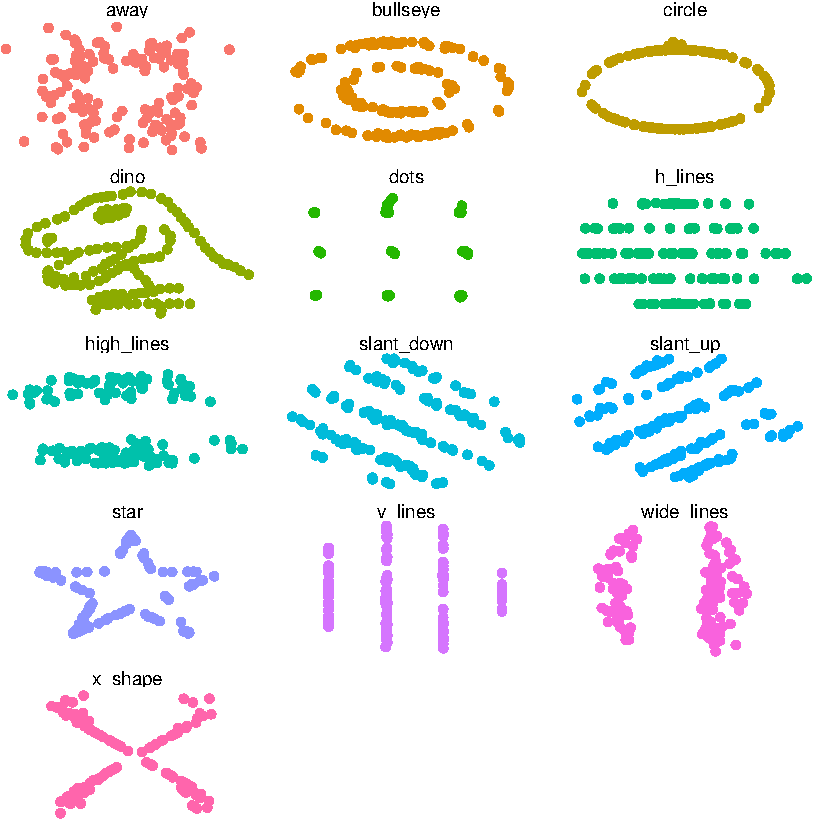
\includegraphics[width=0.5\textwidth,height=\textheight]{_descr_stats_DE_files/figure-pdf/fig-datasauRus-1.pdf}

}

\caption{\label{fig-datasauRus}Plots of datasauRus dataset
distributions}

\end{figure}

\begin{center}\rule{0.5\linewidth}{0.5pt}\end{center}

Stellen Sie Ihre Daten also immer grafisch dar und betrachten Sie nicht
nur die beschreibenden Statistiken!!! Beides ist sehr wichtig für das
Verständnis Ihrer Daten.

\hypertarget{aufgaben}{%
\section{Aufgaben}\label{aufgaben}}

\begin{enumerate}
\def\labelenumi{\arabic{enumi}.}
\tightlist
\item
  Berechnen Sie die Standardabweichung der Werte
  \texttt{152,\ 19,\ 1398,\ 67,\ 2111}, ohne die Funktion \texttt{sd()}
  zu benutzen.

  \begin{itemize}
  \tightlist
  \item
    zeige deine Arbeit. Die folgende R-Syntax könnte nützlich sein (je
    nachdem, wie Sie es machen wollen):

    \begin{itemize}
    \tightlist
    \item
      \texttt{c()}
    \item
      \texttt{Mittelwert()}
    \item
      \texttt{x\^{}2} berechnet das Quadrat eines Wertes (hier,
      \texttt{x})
    \item
      \texttt{sqrt()} berechnet die Quadratwurzel
    \item
      \texttt{Länge()}
    \end{itemize}
  \end{itemize}
\end{enumerate}

\begin{center}\rule{0.5\linewidth}{0.5pt}\end{center}

\begin{enumerate}
\def\labelenumi{\arabic{enumi}.}
\setcounter{enumi}{1}
\tightlist
\item
  Benutze die Funktion \texttt{sd()}, um die Standardabweichung der
  obigen Werte zu drucken. Haben Sie es richtig gemacht?
\item
  Benutze \texttt{summarise}, um den Mittelwert, die Standardabweichung
  und die Anzahl der Beobachtungen für \texttt{dep\_delay} zu drucken.

  \begin{itemize}
  \tightlist
  \item
    Hinweis: Müssen Sie fehlende Werte (\texttt{NA}) entfernen?
  \end{itemize}
\item
  Machen Sie dasselbe, aber fügen Sie das Argument \texttt{.by()} hinzu,
  um die Abfahrtsverzögerung (\texttt{dep\_delay}) pro Monat zu finden

  \begin{itemize}
  \tightlist
  \item
    Ordnen Sie die Ausgabe nach der mittleren Abflugverspätung an.
  \end{itemize}
\item
  Drucke die Ausgabe mit einer schön formatierten Tabelle unter
  Verwendung von \texttt{knitr::kable()} und
  \texttt{kableExtra::kable\_styling())}

  \begin{itemize}
  \tightlist
  \item
    eine Tabellenbeschriftung (\texttt{\#\textbar{}\ label:\ tbl-...})
    und eine Tabellenüberschrift (\texttt{\#\textbar{}\ tbl-cap:})
    einfügen
  \item
    eine Beschreibung der Tabellenergebnisse, einschließlich eines
    Querverweises auf die Tabelle (\texttt{@tbl-...})
  \end{itemize}
\end{enumerate}

\hypertarget{heutige-ziele-1}{%
\section*{Heutige Ziele 🏁}\label{heutige-ziele-1}}

Heute haben wir\ldots{}

\begin{itemize}
\tightlist
\item
  Maße der zentralen Tendenz (neu) kennengelernt ✅
\item
  (Wieder-)Erlernen von Streuungsmaßen ✅
\item
  gelernt, wie man die Funktion \texttt{summarise()} von \texttt{dplyr}
  benutzt ✅
\item
  gelernt, wie man Zusammenfassungen ``nach'' Gruppen erstellt ✅
\end{itemize}

\hypertarget{session-info}{%
\section*{Session Info}\label{session-info}}
\addcontentsline{toc}{section}{Session Info}

Hergestellt mit R version 4.3.0 (2023-04-21) (Already Tomorrow) und
RStudioversion 2023.3.0.386 (Cherry Blossom).

\begin{Shaded}
\begin{Highlighting}[]
\FunctionTok{sessionInfo}\NormalTok{()}
\end{Highlighting}
\end{Shaded}

\begin{verbatim}
R version 4.3.0 (2023-04-21)
Platform: aarch64-apple-darwin20 (64-bit)
Running under: macOS Ventura 13.2.1

Matrix products: default
BLAS:   /Library/Frameworks/R.framework/Versions/4.3-arm64/Resources/lib/libRblas.0.dylib 
LAPACK: /Library/Frameworks/R.framework/Versions/4.3-arm64/Resources/lib/libRlapack.dylib;  LAPACK version 3.11.0

locale:
[1] en_US.UTF-8/en_US.UTF-8/en_US.UTF-8/C/en_US.UTF-8/en_US.UTF-8

time zone: Europe/Berlin
tzcode source: internal

attached base packages:
[1] stats     graphics  grDevices utils     datasets  methods   base     

other attached packages:
 [1] datasauRus_0.1.6 here_1.0.1       lubridate_1.9.2  forcats_1.0.0   
 [5] stringr_1.5.0    dplyr_1.1.2      purrr_1.0.1      readr_2.1.4     
 [9] tidyr_1.3.0      tibble_3.2.1     ggplot2_3.4.2    tidyverse_2.0.0 

loaded via a namespace (and not attached):
 [1] utf8_1.2.3            generics_0.1.3        xml2_1.3.4           
 [4] lattice_0.21-8        stringi_1.7.12        hms_1.1.3            
 [7] digest_0.6.31         magrittr_2.0.3        evaluate_0.21        
[10] grid_4.3.0            timechange_0.2.0      fastmap_1.1.1        
[13] Matrix_1.5-4          rprojroot_2.0.3       jsonlite_1.8.5       
[16] mgcv_1.8-42           httr_1.4.6            rvest_1.0.3          
[19] fansi_1.0.4           viridisLite_0.4.2     scales_1.2.1         
[22] cli_3.6.1             rlang_1.1.1           crayon_1.5.2         
[25] splines_4.3.0         bit64_4.0.5           munsell_0.5.0        
[28] withr_2.5.0           yaml_2.3.7            tools_4.3.0          
[31] parallel_4.3.0        tzdb_0.4.0            colorspace_2.1-0     
[34] webshot_0.5.4         pacman_0.5.1          kableExtra_1.3.4.9000
[37] vctrs_0.6.2           R6_2.5.1              lifecycle_1.0.3      
[40] bit_4.0.5             vroom_1.6.3           pkgconfig_2.0.3      
[43] pillar_1.9.0          gtable_0.3.3          glue_1.6.2           
[46] systemfonts_1.0.4     xfun_0.39             tidyselect_1.2.0     
[49] rstudioapi_0.14       knitr_1.43            farver_2.1.1         
[52] nlme_3.1-162          htmltools_0.5.5       labeling_0.4.2       
[55] svglite_2.1.1         rmarkdown_2.22        compiler_4.3.0       
\end{verbatim}

\hypertarget{literaturverzeichnis}{%
\section*{Literaturverzeichnis}\label{literaturverzeichnis}}

\hypertarget{refs}{}
\begin{CSLReferences}{1}{0}
\leavevmode\vadjust pre{\hypertarget{ref-wickham_r_nodate}{}}%
Wickham, H., Çetinkaya-Rundel, M., \& Grolemund, G. (o.~J.). \emph{R for
{Data Science}} (2. Aufl.). \url{https://r4ds.hadley.nz/}

\end{CSLReferences}



\end{document}
